%% GENERATED by paper/scripts/make_paper_assets.py -- do not edit by hand.
%% source: outputs/train_v3.log + eval/reports/summary.csv
\begin{figure}[t]
\centering
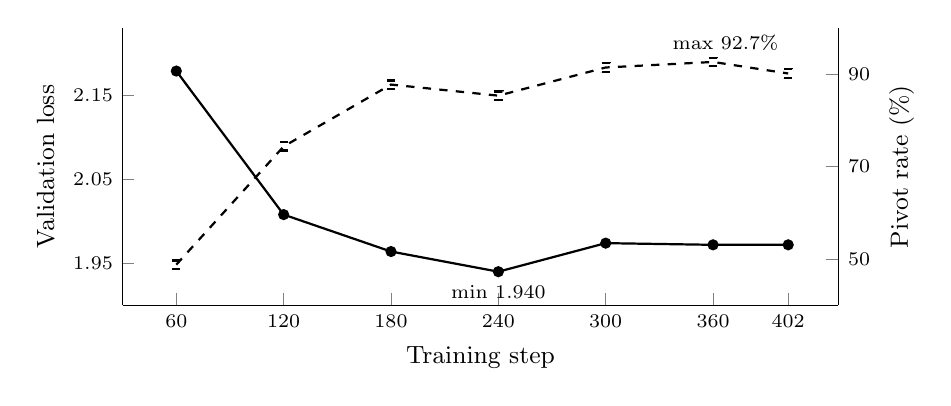
\begin{tikzpicture}
\begin{axis}[
  width=0.88\columnwidth, height=5.1cm,
  xlabel={Training step}, ylabel={Validation loss},
  xmin=30, xmax=430, ymin=1.90, ymax=2.23,
  axis y line*=left, axis x line*=bottom,
  ytick={1.95,2.05,2.15}, xtick={60,120,180,240,300,360,402},
  x tick label style={font=\scriptsize}, y tick label style={font=\scriptsize},
  label style={font=\small},
]
\addplot[thick, mark=*, mark size=1.6pt] coordinates {(60,2.179) (120,2.008) (180,1.964) (240,1.94) (300,1.974) (360,1.972) (402,1.972)};
\node[font=\scriptsize, anchor=north] at (axis cs:240,1.935) {min 1.940};
\end{axis}
\begin{axis}[
  width=0.88\columnwidth, height=5.1cm,
  ylabel={Pivot rate (\%)},
  xmin=30, xmax=430, ymin=40, ymax=100,
  axis y line*=right, axis x line=none,
  ytick={50,70,90},
  y tick label style={font=\scriptsize}, label style={font=\small},
]
\addplot[thick, dashed, mark=square, mark size=1.5pt] coordinates {(60,48.8) (120,74.4) (180,87.8) (240,85.39999999999999) (300,91.5) (360,92.7) (402,90.2)};
\node[font=\scriptsize, anchor=south east] at (axis cs:402,93) {max 92.7\%};
\end{axis}
\end{tikzpicture}
\caption{Loss is uninformative for behavioural checkpoint selection. Validation loss
(solid, left axis) bottoms at step~240 and is flat-to-worse after; the behaviour the model
is being trained for (dashed, right axis) keeps improving to step~360. Early stopping on
loss selects a checkpoint 7.3~points worse on the metric that matters.}
\label{fig:loss}
\end{figure}
